\documentclass{article}

\usepackage{amsmath, tikz, pgfplots, graphicx, float, appendix, listings}
\pgfplotsset{compat=1.7}

% Opening
\title{Drone Package Delivery}
\author{Akash Narayanan}
\date{}

\begin{document}

    \maketitle

    \section{Introduction}
    Suppose you are a recently-hired Amazon employee and you are practicing
    using the delivery drone. In one practice run, the drone starts 5 miles east
    of your home and you aim to fly it directly back home. The drone is
    programmed to travel directly towards your home at a speed of $b$
    mph. However, there is a wind blowing north at a constant $w$ mph.
    Assuming the drone flies at a constant height, we consider how to construct
    a system of differential equations for this situation along with methods for
    modeling and visualizing the drone's trajectory.

    Our approach involves forming a vector equation to represent the drone's
    trajectory, using the information about the velocity the drone experiences
    at various points to derive information about it's instantaneous change in
    position. We analyze various aspects of the system of differential
    equations. We then use this information with modern numerical methods for
    closely approximating solutions to differential equations which may not have
    analytical solutions.

    \section{Analysis}
    We start by visualizing the problem on the 2D plane. We can do so since the
    drone always flies at the same height. Let the origin represent your home
    and the drone will be represented by a point.
    Note that we disregard the dimensions of the drone and treat it as a point
    considering it is miniscule in relation to the distances being considered.

    After translating it to a plane, we may also draw the velocity vectors
    acting on the drone. One of them is the drone's programming, a vector which
    always points towards the origin and has magnitude $b$. The second
    vector constantly points in the positive $y$ direction and has magnitude
    $w$.

    \begin{figure}[H]
        \centering
        \resizebox{10cm}{10cm}{
            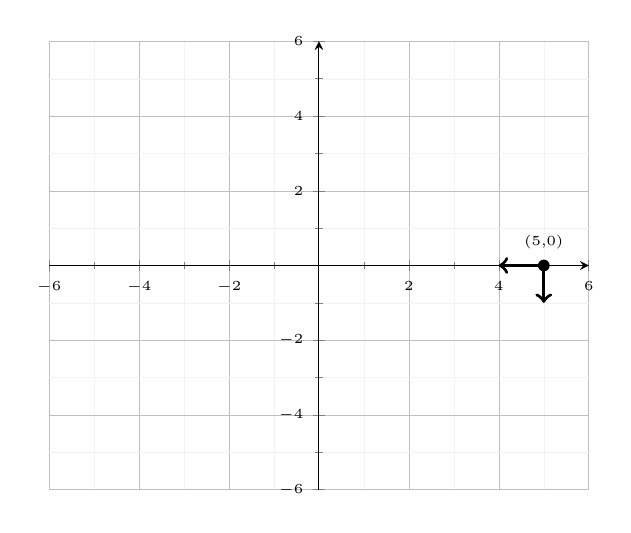
\begin{tikzpicture}
                \begin{axis}[
                    axis lines=middle,
                    xmin=-6, xmax=6,
                    ymin=-6, ymax=6,
                    grid=both,
                    grid style={line width=.1pt, draw=gray!10},
                    major grid style={line width=.2pt, draw=gray!50},
                    minor tick num=1,
                    ticklabel style={font=\tiny}
                    ]
                    \node[label={90:{\tiny{(5,0)}}},circle,fill,inner sep=1.5pt] at
                        (axis cs:5,0) {};
                    \draw[very thick, ->] (axis cs:5,0) -- (axis cs:4,0);
                    \draw[very thick, ->] (axis cs:5,0) -- (axis cs:5,-1);
                \end{axis}
            \end{tikzpicture}
        }
        \caption{\label{fig:graph} A representation of the problem using vectors
        on a plane.}
    \end{figure}

    Using this interpretation, we can construct a set of equations to model the
    drone's motion. Let the drone be at position $(x, y)$. The drone's velocity
    vector points towards the origin and has the direction of the vector $(0, 0)
    - (x, y) = (-x, -y)$. Dividing by its magnitude and multiplying by
    $b$ to reflect the drone's velocity yields the vector
    \[
        v_1 = \frac{(-x, -y)}{\sqrt{x^2 + y^2}} \cdot b
    \] 
    Furthermore, the wind affecting the drone's motion is represented by the
    vector $(0, w)$. Recall that velocity is the derivative of position.
    Combining the two velocity vectors and separating components, we have the
    following non-linear system of differential equations:
    \begin{align}
        x'(t) &= -\frac{bx}{\sqrt{x^2+y^2}} \\
        y'(t) &= -\frac{by}{\sqrt{x^2+y^2}} + w
    \end{align}
    with the initial conditions $x(0) = 5$ and $y(0) = 0$.

    Although there is no obvious analytical solution to this system, we can
    extract some information. For example, consider the nullclines of the
    system. We have
    \[
        -\frac{bx}{\sqrt{x^2+y^2}} = 0
    \] 
    if and only if $x = 0$ and $y \neq 0$. For the  $y$-nullcline, we find
    \[
        -\frac{by}{\sqrt{x^2+y^2}} + w = 0 \\
    \] 
    or
    \[
        \frac{y}{\sqrt{x^2+y^2}} = \frac{w}{b}.
    \] 
    Note that $|y| \leq \sqrt{x^2 + y^2}$ and the equality holds only when $x =
    0$. This implies that the left side of the equality above is contained
    within the range $[-1, 1]$. That is, a $y$-nullcline exists only when $|w|
    \leq |b|$. As a physical interpretation, this is reasonable. It means the
    wind speed must be less than that of the drone's velocity to ensure that
    there is at least one point where the $y$-position of the drone does not
    change instantaneously.

    When the $y$-nullcline does exist, it is given by $y =
    \frac{w}{b}|x|$. Then the only intersection point of the nullclines is at
    the point $(0, 0)$, a point where neither $x'$ nor $y'$ are defined.
    This is reasonable in the context of the problem as the drone would have arrived
    home and there is no need for further motion.

    The slope field for this system with values $b = 6$ and $w = 2$ is shown
    below. It is quite pretty. It is also reasonable to see the trajectory
    corresponding to the given initial position.

%    \begin{center}
%        \includegraphics[width=0.9\textwidth]{media/slopeField.png}
%    \end{center}
    \begin{figure}[H] 
        \centering
        \includegraphics[width=0.8\textwidth]{media/slopeField.png}
        \caption{\label{fig:slope-field-1} The slope field corresponding to
        values $b = 6$, $w = 2$.}
    \end{figure}

    Linearization is not a particularly useful technique here since there are no
    equilibrium solutions and the given initial conditions are far enough away
    from the origin that we can expect any approximations to deviate from an
    actual solution. Instead, we can approximate the solution using a modern
    numerical method, the Runge-Kutta method.

    Although the Runge-Kutta method was initially devised for approximating
    solutions to a single differential equation, it can be expanded to systems
    of equations in a relatively straightforward manner. However, this is
    actually not necessary for our situation because neither of the differential
    equations rely on the parameter $t$. That is, the system is
    autonomous. Therefore, the derivative of the solution curve $dy / dx$ can be
    computed based solely on position and we can implement the Runge-Kutta
    method without having to expand it to several equations.

    Implementing the numerical method in Python and producing a set of points,
    we can plot the approximate trajectory of the drone. Note that we use the
    same constants as in the slope field shown above, namely $b = 6$ and $w =
    2$. The figure below is calculated with 100 steps.

%    \begin{center}
%        \includegraphics[width=0.9\textwidth]{media/overlay.png}
%    \end{center}
    \begin{figure}[H]
        \centering
        \includegraphics[width=0.8\textwidth]{media/overlay.png}
        \caption{\label{fig:overlay} An approximate solution and the
        corresponding slope field.}
    \end{figure}

    Of course, the approximation could be made more accurate with the increasing
    the number of steps and decreasing the step size, or it can be improved by
    evaluating the derivative at more points between each step. However, this
    method provides a curve consistent with the slope field in a very quick
    time.

    It is somewhat interesting to see the results of numerical approximation in
    the case where $|w| > |b|$. Recall that in this case, there are no
    $y$-nullclines. Thus, we should not expect the $y$ position of the drone to
    settle. Indeed, plotting as above with the values $b = 2$ and $w = 3$, we
    find that the drone never reaches home.

%    \begin{center}
%        \includegraphics[width=0.9\textwidth]{media/overlay2.png}
%    \end{center}
    \begin{figure}[H]
        \centering
        \includegraphics[width=0.8\textwidth]{media/overlay2.png}
        \caption{\label{fig:overlay-2} The approximate solution to the problem
        with values $b = 2$, $w = 3$.}
    \end{figure}

    \section{Conclusion}
    Although some initial analysis and reinterpretation of the problem posed was
    required, the system we constructed is quite tame. The ability to
    interchange between a parametric or vector interpretation and a coordinate
    plane enables us to analyze the system. We determined the conditions under
    which the nullclines of the system exist and what they are. Finally, we
    developed a numerical approximation of the solution to the system using the
    Runge-Kutta method discussed in class.

    Although we have effectively solved the problem initially posed, it is worth
    considering variations on the problem. While we only considered a constant
    wind speed, it could be interesting to consider one which varies with
    position. Such a system could still be solved in the same manner as above
    but may yield more interesting nullclines and further analysis.
    Additionally, one could drop the requirement that the system be autonomous
    and consider solutions to the problem if the wind speed or drone speed were
    to change as functions of both time and position.

    \pagebreak

    \begin{thebibliography}{999}
        \bibitem{dronedelivery}
        Eric Stachura; Robert Krueger (2018), "6-024-S-DronePackageDelivery,"
        https://simiode.org/resources/5422.
        
        \bibitem{textbook}
        Trench, William F., "Elementary Differential Equations" (2013).
        \textit{Faculty Authored and Edited Books & CDs.} 8. \\
        https://digitalcommons.trinity.edu/mono/8

        Results in Figure 1 were obtained using the pgfplots package.

        The vector fields in Figures 2, 3, and 4 were obtained using
        https://homepages.bluffton.edu/~nesterd/apps/slopefields.html.

        The graphs obtained in Figures 3 and 4 were created using a Python
        script provided in Appendix 1 and the matplotlib package.
    \end{thebibliography}

    \pagebreak

    \begin{appendices}
        \section{Python Code}
        The following code uses the Runge-Kutta method to generate the points
        found in the table in Appendix 2 and the matplotlib package to generate
        graphs used in above figures.

        \lstinputlisting[language=Python]{runge_kutta.py}

        \section{Tables}
        The following table is a list of points generated by the above Python
        script. These points were used to generate the curves in Figures 3 and
        4.

        \centering
        \begin{tabular}{ |c|c|c| }
            \hline
            Step & $x$ & $y$ \\
            \hline
            0  &  5.00 &  0.00000 \\
            1  &  4.95 &  0.01782 \\
            2  &  4.90 &  0.03545 \\
            3  &  4.85 &  0.05290 \\
            4  &  4.80 &  0.07016 \\
            5  &  4.75 &  0.08723 \\
            \dots & \dots & \dots \\
            95 &  0.25 &  0.18580 \\
            96 &  0.20 &  0.13525 \\
            97 &  0.15 &  0.08127 \\
            98 &  0.10 &  0.03356 \\
            99 &  0.05 &  0.03147 \\
            \hline
        \end{tabular}

    \end{appendices}
\end{document}
